5. \begin{figure}[ht!]
\center{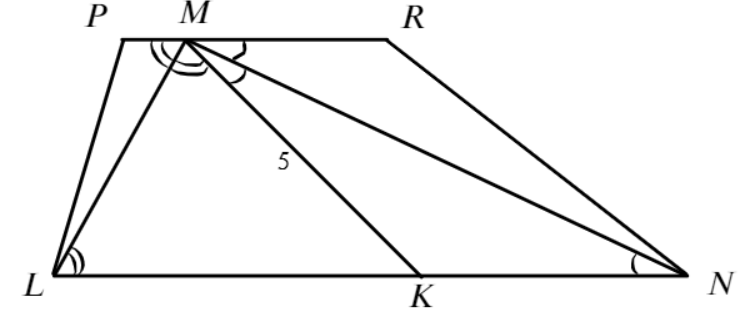
\includegraphics[scale=0.35]{g5.png}}
\end{figure}\\
Прямые $PR$ и $LN$ параллельны, а $LM$ и $MN$ --- секущие, значит $\angle PML = \angle MLK,$  $\angle RMN= \angle MNK$ как накрест лежащие. $MN$ и $ML$ являются биссектрисами, поэтому $\angle PML = \angle LMK,$ $ \angle RMN= \angle NMK.$ Поэтому у треугольников $LMK$ и $NMK$ равны углы при основаниях, а значит они равнобедренные и $LK=MK=5,\ KN=MK=5,$ откуда $LN=LK+KN=5+5=10.$\\
